\section{DEFLATE Algorithm: The Standard in Practice}

\subsection{Introduction: The Universal Compression Standard}

The DEFLATE compression algorithm, specified in RFC 1951 (1996), is arguably the most widely deployed compression algorithm in history. Its success lies not in being the theoretically optimal algorithm, but in striking an exceptional balance between compression ratio, speed, and implementation simplicity.

\begin{definitionbox}
\textbf{DEFLATE}: A lossless data compression algorithm combining LZ77-style string matching with Huffman coding. It is the compression engine behind gzip, ZIP, PNG, and HTTP compression.
\end{definitionbox}

\subsubsection{Where DEFLATE Is Used: gzip, ZIP, PNG, HTTP}

\begin{itemize}
    \item \textbf{gzip}: The Unix compression utility (RFC 1952)
    \item \textbf{ZIP file format}: Phil Katz's PKZIP format (1989), later standardized
    \item \textbf{PNG image format}: Replaced GIF, uses DEFLATE on filtered scanlines
    \item \textbf{HTTP compression}: Content-Encoding: gzip/deflate in web traffic
    \item \textbf{PDF documents}: FlateDecode filter for stream compression
    \item \textbf{Java JAR files}: Based on ZIP format
\end{itemize}

\subsubsection{Historical Context: Phil Katz, ZIP Format, and Open Standards}

The story of DEFLATE is intertwined with the "compression wars" of the late 1980s-1990s:

\begin{itemize}
    \item \textbf{1985}: Terry Welch's LZW algorithm patented (used in GIF)
    \item \textbf{1986}: Phil Katz creates PKARC (based on ARC format)
    \item \textbf{1989}: Katz releases PKZIP with proprietary compression
    \item \textbf{1991}: gzip created as free alternative to UNIX compress (which used LZW)
    \item \textbf{1993}: Unisys enforces LZW patents, creating demand for patent-free alternatives
    \item \textbf{1996}: DEFLATE specification published as RFC 1951
\end{itemize}

The key innovation was making DEFLATE specification \textbf{open} and \textbf{royalty-free}, leading to widespread adoption.

\subsection{High-Level Architecture: A Two-Stage Pipeline}

DEFLATE employs a classic transform-coding approach:

\begin{figure}[H]
\centering
\begin{tikzpicture}[node distance=1.5cm]
\node[draw, rectangle, minimum width=3cm, minimum height=1cm] (input) {Input Data};
\node[draw, rectangle, minimum width=3cm, minimum height=1cm, right=of input] (lzss) {LZSS String Matching};
\node[draw, rectangle, minimum width=3cm, minimum height=1cm, right=of lzss] (huffman) {Huffman Coding};
\node[draw, rectangle, minimum width=3cm, minimum height=1cm, right=of huffman] (output) {Compressed Output};

\draw[->, thick] (input) -- (lzss);
\draw[->, thick] (lzss) -- (huffman);
\draw[->, thick] (huffman) -- (output);

\node[above=0.2cm of lzss] {\textbf{Stage 1: Find Redundancy}};
\node[above=0.2cm of huffman] {\textbf{Stage 2: Encode Efficiently}};
\end{tikzpicture}
\caption{DEFLATE's two-stage compression pipeline}
\end{figure}

\subsubsection{Stage 1: LZSS String Matching (Finding Redundancy)}

The LZSS (Lempel-Ziv-Storer-Szymanski) stage identifies repeated sequences in the data:

\begin{itemize}
    \item Scans input with a \textbf{sliding window} (32KB history buffer)
    \item For each position, looks for longest match in recent history
    \item Outputs either:
    \begin{itemize}
        \item \textbf{Literal byte}: When no good match found
        \item \textbf{(Length, Distance) pair}: When match found
    \end{itemize}
\end{itemize}

\textbf{Example}: For the string "the cat sat on the mat":
\begin{itemize}
    \item First occurrence of "the": output as literals 't','h','e'
    \item Second occurrence of "the": output as (length=3, distance=15)
\end{itemize}

\subsubsection{Stage 2: Huffman Coding (Encoding the Reduced Data)}

The Huffman stage compresses the output from Stage 1:

\begin{itemize}
    \item Takes stream of literals and (length,distance) pairs
    \item Builds \textbf{two Huffman trees}:
    \begin{itemize}
        \item One for literals and lengths (combined alphabet)
        \item One for distances
    \end{itemize}
    \item Uses \textbf{canonical Huffman codes} for compact representation
\end{itemize}

\subsubsection{Why the Hybrid Approach Works: Transforming Redundancy}

The genius of DEFLATE is in how it \textbf{transforms redundancy}:

\begin{enumerate}
    \item \textbf{LZSS finds structural redundancy}: Repeated sequences become (length,distance) pairs
    \item \textbf{Huffman finds statistical redundancy}: Frequent symbols get shorter codes
    \item Together they exploit \textbf{both types} of redundancy in data
\end{enumerate}

\begin{importantbox}
\textbf{Key Insight}: LZSS is excellent at finding \emph{long-range} repetition (phrases, patterns). Huffman is excellent at compressing \emph{skewed distributions}. Together they handle both English text (skewed letter frequencies + repeated words) effectively.
\end{importantbox}

\subsubsection{Design Philosophy: Fast Decoding Over Maximum Compression}

DEFLATE was designed with clear priorities:

\begin{center}
\begin{tabular}{|l|l|}
\hline
\textbf{Priority} & \textbf{Implementation Choice} \\
\hline
Fast decoding & Canonical Huffman (O(1) decode) \\
\hline
Memory efficiency & 32KB sliding window (tiny by today's standards) \\
\hline
Implementation simplicity & Two independent stages \\
\hline
Streaming capability & Independent compression blocks \\
\hline
Acceptable compression & "Good enough" ratio for most data \\
\hline
\end{tabular}
\end{center}

This "fast decode" philosophy made DEFLATE ideal for distribution formats (ZIP, PNG) where files are compressed once but decompressed many times.

\subsection{LZSS in DEFLATE: Detailed Implementation}

\subsubsection{Sliding Window: 32KB History and Lookahead Buffer}

DEFLATE's LZSS uses specific, fixed parameters:

\begin{itemize}
    \item \textbf{History buffer}: 32,768 bytes (2$^{15}$) of recently processed data
    \item \textbf{Lookahead buffer}: 258 bytes maximum match length
    \item \textbf{Minimum match length}: 3 bytes (shorter matches not worth encoding)
\end{itemize}

\begin{examplebox}
\textbf{Why 32KB?}
\begin{itemize}
    \item 32KB was a practical limit in 1990s memory-constrained systems
    \item Larger windows provide diminishing returns for most data
    \item Cache-friendly size for modern processors
    \item Still adequate for most short-to-medium range repetitions
\end{itemize}
\end{examplebox}

\subsubsection{Hash Chains for Fast Match Finding}

Instead of brute-force searching 32KB for matches, DEFLATE uses a hash table:

\begin{algorithm}[H]
\caption{DEFLATE Match Finding with Hash Chains}
\begin{algorithmic}[1]
\Procedure{FindBestMatch}{$current\_position$, $data$}
\State $hash \gets \text{hash}(data[current\_position:current\_position+3])$
\State $best\_length \gets 0$
\State $best\_distance \gets 0$
\For{each $prev\_pos$ in $hash\_table[hash]$}
    \If{$current\_pos - prev\_pos > 32768$} \Comment{Outside window}
        \State \textbf{continue}
    \EndIf
    \State $length \gets \text{MatchLength}(prev\_pos, current\_pos)$
    \If{$length > best\_length$}
        \State $best\_length \gets length$
        \State $best\_distance \gets current\_pos - prev\_pos$
    \EndIf
\EndFor
\State \textbf{return} $(best\_length, best\_distance)$
\EndProcedure
\end{algorithmic}
\end{algorithm}

The hash is typically computed from the first 3 bytes of the potential match. Hash chains link all positions with the same 3-byte prefix.

\subsubsection{Lazy Matching and Greedy Heuristics}

DEFLATE uses sophisticated heuristics to find better matches:

\begin{itemize}
    \item \textbf{Greedy parsing}: Take the longest match at current position
    \item \textbf{Lazy evaluation}: Check if skipping 1 byte finds a better match
    \item \textbf{Lazy matching}: Actually implement lazy evaluation
\end{itemize}

\begin{examplebox}
\textbf{Lazy Matching Example:}
Data: "abcdeabcdfabcde"

\begin{enumerate}
    \item At position 0: "abcde" matches at position 5 (length=5)
    \item \textbf{Greedy}: Encode (length=5, distance=5) immediately
    \item \textbf{Lazy}: Check position 1: "bcdeabcdfabcde" has match at position 6 (length=13)
    \item Better! So output 'a' as literal, then encode long match
\end{enumerate}

Lazy matching finds longer matches but requires more computation.
\end{examplebox}

\subsubsection{Output Format: (Length, Distance) Pairs vs. Literal Bytes}

The LZSS stage produces a stream of symbols from two alphabets:

\begin{center}
\begin{tabular}{|l|l|l|}
\hline
\textbf{Type} & \textbf{Range} & \textbf{Encoding Details} \\
\hline
Literal bytes & 0--255 & Direct byte values \\
\hline
Length codes & 3--258 & Base code + 0--5 extra bits for longer lengths \\
\hline
Distance codes & 1--32768 & Base code + 0--13 extra bits in logarithmic ranges \\
\hline
End-of-block & 256 & Special marker (end of DEFLATE block) \\
\hline
\end{tabular}
\end{center}

\textbf{Important encoding details:}

\begin{itemize}
    \item \textbf{Lengths 3--258}: Encoded using symbols 257--285
    \begin{itemize}
        \item For example: Length 3 = symbol 257 (no extra bits)
        \item Length 10 = symbol 264 (no extra bits)
        \item Length 258 = symbol 285 (no extra bits)
        \item Lengths 11--258 use 1--5 extra bits for precise encoding
    \end{itemize}
    
    \item \textbf{Distances 1--32768}: Encoded using symbols 0--29 with logarithmic ranges
    \begin{itemize}
        \item Example ranges:
        \begin{itemize}
            \item Symbol 0: Distance 1 (no extra bits)
            \item Symbol 4: Distances 5--6 (1 extra bit)
            \item Symbol 29: Distances 24577--32768 (13 extra bits)
        \end{itemize}
        \item Distance 100 would use symbol for range 97--128 with extra bits
    \end{itemize}
\end{itemize}

\begin{examplebox}
\textbf{Encoding Distance 100:}
\begin{enumerate}
    \item Distance 100 falls in range 97--128
    \item According to DEFLATE specification:
    \begin{itemize}
        \item Range 97--128 corresponds to distance symbol 18
        \item Base distance for this symbol: 97
        \item Extra bits needed: 2 bits (since 128-97+1 = 32 possibilities)
    \end{itemize}
    \item Compute extra bits: 100 - 97 = 3
    \item Encode as: symbol 18 followed by binary '11' (3 in 2 bits)
\end{enumerate}
\end{examplebox}

This logarithmic encoding allows representing 32768 possible distances with only 30 symbols plus extra bits, significantly reducing the Huffman alphabet size.

\subsection{DEFLATE's Unique Huffman Coding Scheme}

This is where DEFLATE shows its brilliance. Instead of storing full Huffman trees, it stores only \textbf{code lengths}.

\subsubsection{Two Alphabets: Literals (0-285) and Distances (0-29)}

DEFLATE uses separate Huffman trees for different symbol types:

\begin{itemize}
    \item \textbf{Literals/Lengths alphabet}: 286 symbols
    \begin{itemize}
        \item 0-255: Literal bytes
        \item 256: End-of-block marker
        \item 257-285: Length codes (with extra bits)
    \end{itemize}
    
    \item \textbf{Distances alphabet}: 30 symbols
    \begin{itemize}
        \item 0-3: Direct distances 1-4
        \item 4-29: Distance codes with extra bits
    \end{itemize}
\end{itemize}

\subsubsection{Canonical Huffman via Code Lengths: The Brilliant Compression}

Instead of storing:
\begin{itemize}
    \item Full tree structure (large), or
    \item Symbol-to-code mapping (variable size)
\end{itemize}

DEFLATE stores only:
\begin{itemize}
    \item \textbf{Code length for each symbol} (4 bits each, 19 maximum length)
    \item \textbf{Canonical reconstruction rules}:
    \begin{enumerate}
        \item Sort symbols by code length
        \item Assign first code of length $k$ as 0
        \item Each subsequent code = previous code + 1
        \item When increasing length, left-shift and add zeros
    \end{enumerate}
\end{itemize}

\begin{examplebox}
\textbf{Canonical Huffman Example:}

Given code lengths: A=2, B=2, C=3, D=3, E=3

\begin{enumerate}
    \item Sort by length: A(2), B(2), C(3), D(3), E(3)
    \item Length 2: Start with 00
    \item Assign: A=00, B=01 (00+1)
    \item Length 3: Start with 100 (01<<1)
    \item Assign: C=100, D=101, E=110
\end{enumerate}

Decoder only needs code lengths to reconstruct this!
\end{examplebox}

\subsubsection{Run-Length Encoding of Code Lengths (19-Symbol Alphabet)}

Code lengths themselves are compressed using RLE on a 19-symbol alphabet:

\begin{itemize}
    \item 0-15: Actual code length 0-15
    \item 16: Repeat previous length 3-6 times (2 extra bits)
    \item 17: Repeat zero 3-10 times (3 extra bits)
    \item 18: Repeat zero 11-138 times (7 extra bits)
\end{itemize}

This compression means the Huffman tree description is itself heavily compressed!

\subsubsection{Why Canonical Codes Enable O(1) Decoding}

With canonical codes, decoding becomes a table lookup:

\begin{lstlisting}[language=C, caption=Canonical Huffman Decoding (Pseudocode)]
// Precomputed tables from code lengths
min_code[length] = smallest code of this length
max_code[length] = largest code of this length
first_symbol[length] = first symbol with this length

// Decoding loop
while (need more symbols) {
    code = peek_bits(MAX_BITS);  // Look at next bits
    for (len = 1 to MAX_BITS) {
        if (code <= max_code[len]) {
            symbol = first_symbol[len] + (code - min_code[len]);
            consume_bits(len);
            break;
        }
    }
}
\end{lstlisting}

This is \textbf{O(1)} per symbol (constant-time lookup), crucial for fast decompression.

\subsection{Block Structure and Streaming Format}

DEFLATE supports streaming through independent compression blocks.

\subsubsection{Three Block Types: Stored, Fixed Huffman, Dynamic Huffman}

\begin{center}
\begin{tabular}{|l|l|l|}
\hline
\textbf{Type} & \textbf{Bits} & \textbf{Use Case} \\
\hline
\textbf{Stored} & 00 & Uncompressible data \\
\hline
\textbf{Fixed Huffman} & 01 & Default trees (predefined) \\
\hline
\textbf{Dynamic Huffman} & 10 & Custom trees per block \\
\hline
\textbf{Reserved} & 11 & (Error) \\
\hline
\end{tabular}
\end{center}

\begin{itemize}
    \item \textbf{Stored blocks}: Raw data with length header (for already-compressed data)
    \item \textbf{Fixed blocks}: Use predefined Huffman trees (no tree description overhead)
    \item \textbf{Dynamic blocks}: Custom optimized trees (best compression)
\end{itemize}

\subsubsection{Bit-Level Layout: BFINAL, BTYPE, and Data}

Each block has precise bit-level layout:

\begin{lstlisting}[language=C, caption=DEFLATE Block Structure]
// Block header
BFINAL: 1 bit  (1 = last block in stream)
BTYPE:  2 bits (00, 01, or 10)

// If BTYPE == 00 (Stored block)
//    Skip to next byte boundary
//    LEN: 16 bits (block length)
//    NLEN: 16 bits (~LEN for error checking)
//    Data: LEN bytes of raw data

// If BTYPE == 01 (Fixed Huffman)
//    Compressed data using fixed trees

// If BTYPE == 10 (Dynamic Huffman)
//    HLIT: 5 bits (257-286 literal/length codes)
//    HDIST: 5 bits (1-30 distance codes)
//    HCLEN: 4 bits (4-19 code length codes)
//    Code lengths for code length alphabet (HCLEN+4 times)
//    Compressed literal/length and distance code lengths
//    Compressed data
\end{lstlisting}

\subsubsection{Streaming Support: Independent Blocks and Reset Points}

\begin{itemize}
    \item Each block compressed independently
    \item History buffer \textbf{does not reset} between blocks (maintains 32KB window)
    \item Allows streaming compression of unlimited data
    \item Enables random access in some formats (ZIP seeks to file boundaries)
\end{itemize}

\subsection{Step-by-Step Compression Walkthrough}

Let's trace through compressing a simple English phrase.

\subsubsection{Input: "The cat sat on the mat"}

Assume ASCII encoding (simplified for example):
\begin{verbatim}
Position: 012345678901234567890123456
Text:     The cat sat on the mat
Indices:  0         1         2
\end{verbatim}

\subsubsection{LZSS Processing: Finding Matches}

\begin{enumerate}
    \item Position 0-2: "The" - No match in empty history → Output literals 'T','h','e'
    \item Position 3: ' ' (space) - No match → Output literal ' '
    \item Position 4-6: "cat" - No match → Output 'c','a','t'
    \item Continue... Position 18-20: "the" matches position 0-2!
    \item Match length = 3, distance = 18
    \item Encode as (length=3, distance=18)
\end{enumerate}

Final LZSS output (simplified):
\begin{verbatim}
Literals: T h e   c a t   s a t   o n   (length,distance=3,18) m a t
Symbols: 84 104 101 32 99 97 116 32 115 97 116 32 111 110 (257,18) 109 97 116
\end{verbatim}

(Note: 257 is the symbol for length=3 in DEFLATE's encoding)

\subsubsection{Building Canonical Huffman Tables}

From the symbol stream, compute frequencies:

\begin{center}
\begin{tabular}{|l|l|}
\hline
\textbf{Symbol} & \textbf{Frequency} \\
\hline
32 (space) & 4 \\
\hline
97 ('a') & 3 \\
\hline
116 ('t') & 3 \\
\hline
Others & 1 each \\
\hline
257 (length=3) & 1 \\
\hline
18 (distance) & 1 \\
\hline
\end{tabular}
\end{center}

Build Huffman trees, then extract code lengths. For example, space (32) gets shortest code.

\subsubsection{Bitstream Assembly: Final Compressed Output}

\begin{enumerate}
    \item Write block header: BFINAL=1, BTYPE=10 (dynamic)
    \item Write HLIT, HDIST, HCLEN values
    \item Write compressed code lengths for the 19 code-length symbols
    \item Write compressed literal/length and distance code lengths
    \item Write compressed data using the Huffman codes
    \item Pad final byte with zeros if needed
\end{enumerate}

\subsection{Compression Levels and Performance Trade-offs}

zlib (the reference implementation) offers 9 compression levels.

\subsubsection{zlib's 9 Levels: From "fast" to "best"}

\begin{center}
\begin{tabular}{|l|l|l|}
\hline
\textbf{Level} & \textbf{Strategy} & \textbf{Use Case} \\
\hline
0 & No compression (store only) & Testing/disabled \\
\hline
1 & Fastest LZ77, lazy matching off & Real-time compression \\
\hline
6 & Default: moderate search, lazy matching & General purpose \\
\hline
9 & Full search, optimal parsing & Archival storage \\
\hline
\end{tabular}
\end{center}

Levels mainly differ in:
\begin{itemize}
    \item Hash table size and chain length
    \item Lazy matching on/off
    \item Match selection heuristics
\end{itemize}

\subsubsection{Speed vs. Ratio: Why Level 6 is the Default}

The default level 6 represents the "knee" in the speed/ratio curve:

\begin{figure}[H]
\centering
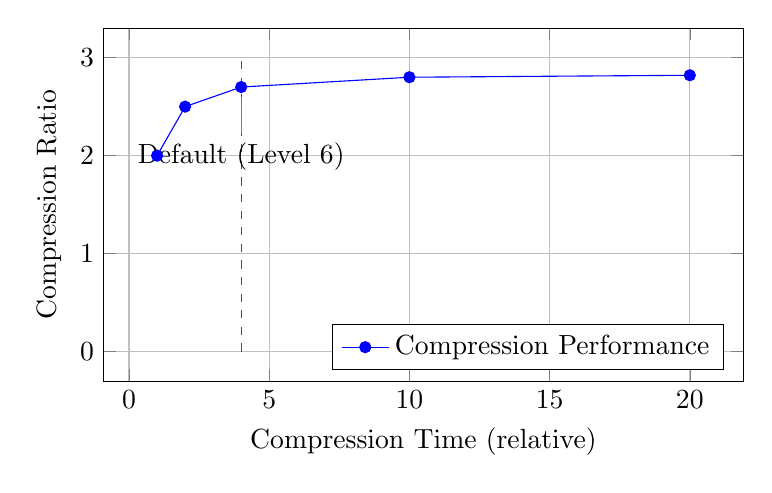
\begin{tikzpicture}
\begin{axis}[
    xlabel={Compression Time (relative)},
    ylabel={Compression Ratio},
    grid=major,
    width=0.8\textwidth,
    height=0.5\textwidth,
    legend pos=south east,
]
\addplot[mark=*, blue] coordinates {
    (1, 2.0) % Level 1
    (2, 2.5) % Level 3
    (4, 2.7) % Level 6 (default)
    (10, 2.8) % Level 9
    (20, 2.82) % Maximum
};
\addplot[red, dashed] coordinates {(4, 0) (4, 3)};
\node[pin=270:{Default (Level 6)}] at (axis cs:4,2.7) {};
\legend{Compression Performance}
\end{axis}
\end{tikzpicture}
\caption{Trade-off between compression time and ratio in zlib}
\end{figure}

Level 9 is only ~5\% better than Level 6 but takes 2-5x longer.

\subsubsection{Memory Footprint: 32KB to 256KB Windows}

\begin{itemize}
    \item \textbf{Default}: 32KB history buffer + 16KB hash table ≈ 48KB
    \item \textbf{Maximum}: Some implementations allow 256KB windows
    \item \textbf{Modern systems}: Typically use 32KB-64KB for cache efficiency
\end{itemize}

\subsection{Practical Applications and File Formats}

\subsubsection{gzip Format: Headers, Footers, and CRC32}

A gzip file contains:
\begin{verbatim}
+--------+------+------+-----+------+------+-------+------+
| Header | Extra| Name |Comment|HCRC | DEFLATE | CRC32 | ISIZE |
+--------+------+------+-----+------+------+-------+------+
  10 bytes optional optional 2    compressed  4      4
\end{verbatim}

\begin{itemize}
    \item \textbf{Header}: Magic bytes (0x1F, 0x8B), compression method (8=DEFLATE)
    \item \textbf{CRC32}: 32-bit checksum of uncompressed data
    \item \textbf{ISIZE}: Uncompressed size modulo 2$^{32}$
\end{itemize}

\subsubsection{ZIP Format: Multiple Files and DEFLATE}

ZIP is a container format supporting multiple compression methods:
\begin{itemize}
    \item Each file compressed independently with DEFLATE
    \item Central directory at end enables random access
    \item Supports encryption, comments, extra fields
\end{itemize}

\subsubsection{PNG: DEFLATE on Filtered Scanlines}

PNG applies a \textbf{filter} to each scanline before DEFLATE:
\begin{itemize}
    \item Subtract pixel from left pixel (Sub filter)
    \item Subtract pixel from above pixel (Up filter)
    \item Various predictors to create more compressible data
    \item Then DEFLATE compresses the filtered bytes
\end{itemize}

\subsubsection{HTTP Compression: Accept-Encoding Header}

Web servers compress responses on-the-fly:
\begin{verbatim}
Request:  GET /page.html HTTP/1.1
          Accept-Encoding: gzip, deflate
          
Response: HTTP/1.1 200 OK
          Content-Encoding: gzip
          [gzip-compressed body]
\end{verbatim}

Saves 60-80\% bandwidth for text content (HTML, CSS, JS).

\subsection{Limitations and When DEFLATE Fails}

\subsubsection{Poor Performance on Already-Compressed or Random Data}

\begin{itemize}
    \item \textbf{Already compressed}: JPEG, MP3, ZIP files → DEFLATE can't compress further
    \item \textbf{Encrypted data}: Random-looking → No patterns to find
    \item \textbf{Result}: May actually \emph{increase} size due to overhead
\end{itemize}

Good compressors detect this and use "stored" (uncompressed) blocks.

\subsubsection{The "Shakespeare Problem": Global vs. Local Repetition}

DEFLATE's 32KB window can't capture \textbf{global repetition}:

\begin{examplebox}
\textbf{Shakespeare's Complete Works:}
\begin{itemize}
    \item Word "the" appears thousands of times
    \item But only instances within 32KB of each other are linked
    \item Distant repetitions (across chapters) aren't captured
    \item Result: Compresses to ~2 bits/byte instead of potential ~1.5
\end{itemize}
\end{examplebox}

Modern compressors (LZMA, zstd) use larger dictionaries (MBs) for this case.

\subsubsection{Why Not Arithmetic Coding? Patents, Speed, and Complexity}

In the 1990s, arithmetic coding was:
\begin{itemize}
    \item \textbf{Patented}: IBM held key patents
    \item \textbf{Slower}: 2-10x slower than Huffman
    \item \textbf{Complex}: Harder to implement correctly
    \item \textbf{Bit-level operations}: Unfriendly to byte-oriented systems
\end{itemize}

Today, arithmetic coding is patent-free but DEFLATE's ecosystem is entrenched.

\subsubsection{Security Issues: CRIME, BREACH, and Compression Side-Channels}

Compression can leak information:
\begin{itemize}
    \item \textbf{CRIME (2012)}: HTTPS compression reveals session cookies
    \item \textbf{BREACH (2013)}: HTTP compression reveals CSRF tokens
    \item \textbf{Principle}: If secret affects compressed size, attacker can deduce it
    \item \textbf{Solution}: Disable compression on sensitive data or use random padding
\end{itemize}

\subsection{Modern Alternatives and Successors}

\subsubsection{LZMA and 7-Zip: Better Compression, Slower Speed}

LZMA (Lempel-Ziv-Markov chain Algorithm):
\begin{itemize}
    \item \textbf{Larger window}: Up to 4GB vs DEFLATE's 32KB
    \item \textbf{Range coding}: Arithmetic coding variant
    \item \textbf{Better compression}: 30-50\% smaller than DEFLATE
    \item \textbf{Slower}: 5-10x slower compression
    \item \textbf{Used in}: 7z format, xz utilities, software installers
\end{itemize}

\subsubsection{Zstandard (zstd): Facebook's Balanced Alternative}

zstd (2016) aims to replace DEFLATE:
\begin{itemize}
    \item \textbf{Faster}: 5-10x faster decompression than zlib
    \item \textbf{Better compression}: 10-20\% better than zlib at same speed
    \item \textbf{Modern features}: Dictionary training, reproducible builds
    \item \textbf{Adoption}: Linux kernel, SquashFS, Facebook, Netflix
\end{itemize}

\subsubsection{Brotli: Google's Web-Optimized Successor}

Brotli (2013) targets web compression:
\begin{itemize}
    \item \textbf{Static dictionary}: 120KB of common web strings
    \item \textbf{Better text compression}: 20-26\% better than gzip
    \item \textbf{Slower compression}: But fast decompression
    \item \textbf{Adoption}: CDNs, web servers, browsers
\end{itemize}

\subsubsection{Why DEFLATE Still Dominates: The Legacy Effect}

Despite better alternatives, DEFLATE persists because:
\begin{itemize}
    \item \textbf{Ubiquitous support}: Every system has zlib
    \item \textbf{Standardized}: RFC 1951, no licensing issues
    \item \textbf{Good enough}: For most use cases
    \item \textbf{Network effects}: Hard to change entrenched standards
    \item \textbf{Hardware support}: Some processors have DEFLATE acceleration
\end{itemize}

\subsection{Hands-On Analysis and Debugging}

\subsubsection{Using gzip -v -l and infgen for Inspection}

\begin{lstlisting}[language=bash]
# Basic compression
gzip -9 file.txt              # Maximum compression
gzip -1 file.txt              # Fastest compression

# Analyze compressed file
gzip -l file.txt.gz           # List compression ratio
gzip -v -l file.txt.gz        # Verbose listing

# Decompress with verbose output
gzip -v -d file.txt.gz        # Show compression ratio

# Use infgen for detailed DEFLATE analysis
infgen -d file.gz             # Disassemble DEFLATE stream
\end{lstlisting}

\subsubsection{Visualizing Matches and Huffman Trees}

Tools for deeper analysis:
\begin{itemize}
    \item \textbf{puff}: Educational DEFLATE implementation (readable C)
    \item \textbf{infgen}: DEFLATE stream disassembler
    \item \textbf{Custom scripts}: Parse zlib output with ZLIB\_DEBUG
\end{itemize}

\subsubsection{Benchmarking: Compression Ratio vs. Speed}

\begin{lstlisting}[language=bash]
# Time compression
time gzip -9 large_file.txt

# Compare compression levels
for level in {1..9}; do
    echo -n "Level $level: "
    gzip -c -$level file.txt | wc -c
done

# Benchmark suite
pigz                 # Parallel gzip implementation
zstd -b              # zstd benchmark mode
\end{lstlisting}

\subsection{Summary and Key Insights}

\subsubsection{Why DEFLATE Dominated for 30+ Years}

\begin{enumerate}
    \item \textbf{Right trade-offs}: Fast decode over maximum compression
    \item \textbf{Clever engineering}: Canonical Huffman, compact tree representation
    \item \textbf{Open standard}: RFC 1951, no patents, reference implementation
    \item \textbf{Good enough}: Adequate compression for most real-world data
    \item \textbf{Ecosystem}: Tools, libraries, hardware support
\end{enumerate}

\subsubsection{Lessons for Compression Engineers: Practical Beats Perfect}

\begin{itemize}
    \item \textbf{Decode speed matters more than encode speed} for distribution formats
    \item \textbf{Implementation simplicity} leads to wider adoption
    \item \textbf{Open standards} defeat technically superior proprietary formats
    \item \textbf{Backward compatibility} is a powerful force
    \item Sometimes \textbf{"good enough" wins over "best"}
\end{itemize}

\subsubsection{Looking Forward: The Future of Compression Standards}

\begin{itemize}
    \item \textbf{DEFLATE will persist} in legacy systems for decades
    \item \textbf{zstd and Brotli} gaining ground in new applications
    \item \textbf{Hardware acceleration} becoming common (Intel QAT, AWS Nitro)
    \item \textbf{AI/ML approaches} showing promise but not yet practical
    \item The next "DEFLATE" will need to be \textbf{10x better} to displace it
\end{itemize}

\begin{importantbox}
\textbf{Final Thought}: DEFLATE represents a peak in practical algorithm design. It shows how understanding both theory (information theory) and practice (hardware constraints, use cases) leads to enduring solutions. Study DEFLATE not just to use it, but to learn how to design algorithms that stand the test of time.
\end{importantbox}

\subsection*{End of Chapter Exercises}

\begin{exercisebox}
\textbf{Exercise 6.1: DEFLATE Architecture Understanding}

Explain in your own words why DEFLATE uses a two-stage approach (LZSS + Huffman) instead of just one of these techniques. Consider:
\begin{enumerate}[label=(\alph*)]
    \item What types of redundancy does LZSS exploit that Huffman cannot?
    \item What types of redundancy does Huffman exploit that LZSS cannot?
    \item Why can't Huffman coding alone achieve good compression on typical text data?
    \item Why can't LZSS alone achieve optimal compression?
\end{enumerate}
\end{exercisebox}

\begin{exercisebox}
\textbf{Exercise 6.2: LZSS Match Analysis}

Given the input string: "abracadabraabracadabra"
\begin{enumerate}[label=(\alph*)]
    \item Using a sliding window of size 12, trace through LZSS processing and show the output as a sequence of literals and (length, distance) pairs.
    \item Calculate the compression ratio if literals are 8 bits and each (length, distance) pair requires 24 bits (8 for length, 16 for distance).
    \item What would be the output if the sliding window was only size 6 instead of 12?
\end{enumerate}
\end{exercisebox}

\begin{exercisebox}
\textbf{Exercise 6.3: Distance Encoding Practice}

Using DEFLATE's distance encoding scheme (logarithmic ranges):
\begin{enumerate}[label=(\alph*)]
    \item Encode the following distances: 1, 5, 10, 100, 1000, 20000
    \item For each, specify: symbol number, base distance, extra bits required, and final binary encoding.
    \item What is the maximum distance that can be encoded without extra bits?
    \item Why does DEFLATE use logarithmic encoding instead of direct binary representation?
\end{enumerate}

\textit{Hint: Refer to RFC 1951 Section 3.2.5 for the exact distance code table.}
\end{exercisebox}

\begin{exercisebox}
\textbf{Exercise 6.4: Canonical Huffman Construction}

Given the following symbol frequencies for a small alphabet:
\begin{center}
\begin{tabular}{|c|c|}
\hline
\textbf{Symbol} & \textbf{Frequency} \\
\hline
A & 40 \\
B & 30 \\
C & 15 \\
D & 10 \\
E & 5 \\
\hline
\end{tabular}
\end{center}

\begin{enumerate}[label=(\alph*)]
    \item Build a Huffman tree and determine code lengths for each symbol.
    \item Generate the canonical Huffman codes from these lengths.
    \item Show the exact bit sequence DEFLATE would store to represent these code lengths.
    \item Calculate the average code length and compare it to the entropy.
\end{enumerate}
\end{exercisebox}

\begin{exercisebox}
\textbf{Exercise 6.5: DEFLATE Block Analysis}

Consider the following DEFLATE block header (in binary):
\[
1\ 10\ 01101\ 00101\ 0100
\]
Where the bits represent: BFINAL (1), BTYPE (10), HLIT (5 bits), HDIST (5 bits), HCLEN (4 bits).

\begin{enumerate}[label=(\alph*)]
    \item Decode each field and explain what it means.
    \item What type of block is this?
    \item How many literal/length codes will follow?
    \item How many distance codes will follow?
    \item How many code-length codes will follow?
\end{enumerate}
\end{exercisebox}

\begin{exercisebox}
\textbf{Exercise 6.6: Compression Level Trade-offs}

You are designing a compression system for:
\begin{enumerate}[label=(\alph*)]
    \item A web server compressing HTML pages in real-time
    \item An archival system storing historical documents
    \item A mobile app with limited CPU and battery
\end{enumerate}

For each scenario:
\begin{itemize}
    \item Recommend a DEFLATE compression level (0-9) with justification
    \item Explain whether you would use fixed or dynamic Huffman blocks
    \item Discuss any modifications you might make to the standard DEFLATE parameters
\end{itemize}
\end{exercisebox}

\begin{exercisebox}
\textbf{Exercise 6.7: DEFLATE vs. Modern Alternatives}

Compare DEFLATE with two modern alternatives (choose from LZMA, zstd, or Brotli):
\begin{enumerate}[label=(\alph*)]
    \item Create a comparison table covering: compression ratio, speed (encode/decode), memory usage, and typical use cases.
    \item For each of the following, recommend which compressor to use and why:
    \begin{itemize}
        \item Compressing software updates for download
        \item Real-time compression in a database
        \item Web assets on a content delivery network
    \end{itemize}
    \item Explain why DEFLATE is still widely used despite newer, better algorithms.
\end{enumerate}
\end{exercisebox}

\begin{exercisebox}
\textbf{Exercise 6.8: Implementation Challenge}

Write pseudocode for a DEFLATE decoder that:
\begin{enumerate}[label=(\alph*)]
    \item Reads the block header and identifies block type
    \item For dynamic blocks, reconstructs the Huffman trees from code lengths
    \item Decodes the compressed data using canonical Huffman decoding
    \item Handles both literals and (length, distance) pairs
\end{enumerate}

Focus on the key algorithms, not edge cases or optimizations. Your pseudocode should show the overall structure and critical steps.
\end{exercisebox}

\begin{exercisebox}
\textbf{Exercise 6.9: Security Analysis}

The CRIME and BREACH attacks exploit compression side-channels:
\begin{enumerate}[label=(\alph*)]
    \item Explain the fundamental vulnerability that enables these attacks.
    \item Why does DEFLATE's LZSS stage make this vulnerability particularly dangerous?
    \item Propose three different strategies to mitigate this risk while still using compression.
    \item Would switching to a different compression algorithm (like zstd or Brotli) solve the problem? Why or why not?
\end{enumerate}
\end{exercisebox}

\begin{exercisebox}
\textbf{Exercise 6.10: Research and Reflection}

\begin{enumerate}[label=(\alph*)]
    \item DEFLATE was standardized in 1996. Identify three technological constraints from that era that influenced DEFLATE's design decisions.
    \item If you were designing DEFLATE today, what would you change given modern hardware (multi-core CPUs, gigabytes of RAM, SSD storage)?
    \item Research the current state of hardware-accelerated compression (Intel QAT, AWS Nitro, etc.). How might these technologies change the optimal compression algorithm design?
    \item Predict: Will DEFLATE still be widely used in 2030? Justify your answer.
\end{enumerate}
\end{exercisebox}

\begin{importantbox}
\textbf{Exercise Guidelines:}
\begin{itemize}
    \item \textbf{Exercises 6.1-6.5}: Core concepts – recommended for all students
    \item \textbf{Exercises 6.6-6.8}: Intermediate application – for deeper understanding
    \item \textbf{Exercises 6.9-6.10}: Advanced topics – for interested students or projects
    \item \textbf{Time estimates}: Basic exercises (30 min each), advanced (60-90 min each)
    \item \textbf{Resources}: Refer to RFC 1951, zlib source code, and infgen tool for hands-on exploration
\end{itemize}
\end{importantbox}

\begin{tcolorbox}[colback=yellow!5!white,colframe=yellow!75!black,title=Optional Project Challenge]
\textbf{Build a Simple DEFLATE Analyzer:}
Write a program in your preferred language that:
\begin{itemize}
    \item Takes a gzip file as input
    \item Parses the gzip header and trailer
    \item Extracts the DEFLATE stream
    \item Identifies block boundaries and types
    \item Reports basic statistics (compression ratio, block types used, etc.)
    \item \textbf{Bonus}: Visualize the Huffman trees or match distances
\end{itemize}
Use existing libraries for decompression, but implement the analysis logic yourself. This project will deepen your understanding of the actual byte-level format.
\end{tcolorbox}
